\section{Experiments}
\label{sec:experiments}
We implemented our solver in \textsc{Julia} and our code is available at \href{https://github.com/EnricoBarbieri1997/cylinder-based-homotopy-camera-calibration}{Github}. Accuracy and robustness are assessed in a synthetic controlled scenario, on a digital replica of a real setting, and in two scenarios where real photographs of the scene were taken.

\subsection{Synthetic experiments}

We generated 50 different synthetic configurations consisting of $N = 2$ cameras and $M = 3$ cylinders. The cylinders are placed in general 3D positions, while all cameras share the same intrinsic matrix $\KK$ and are also positioned generically in space, with their optical axes oriented toward the barycenter of the cylinders.
We evaluate the performance of our method on the two tasks of camera calibration and camera pose estimation.
As regard camera calibration, we consider the relative errors $\Delta f, \Delta c$ and $\Delta s$ on focal lenghts, principal point and skew. In formulas:
\begin{equation}
\Delta f = \frac{1}{2}\frac{|f_x-\overline{f_x}|}{\overline{f_x}}+\frac{1}{2}\frac{|f_y-\overline{f_y}|}{\overline{f_y}},\quad 
\Delta c = \frac{1}{2}\frac{|c_x-\overline{c_x}|}{|\overline{c_x}|}+\frac{1}{2}\frac{|c_y-\overline{c_y}|}{|\overline{c_y}|}, \quad
 \Delta \alpha = \frac{|\alpha-\overline{\alpha}|}{\overline{\alpha}}.
\end{equation}
Poses are evaluated in terms of a rotation error in degree $\Delta \RR$ and a transaltion error $\Delta \mathbf{t}$:
\begin{equation}
 \Delta \RR = \cos^{-1}\left(\frac{\mathrm{trace}(\RR \overline{\RR}^\top) - 1}{2} \right),\quad
  \Delta \mathbf{t} = \frac{||\mathbf{t}-\overline{\mathbf{t}}||}{||\overline{\mathbf{t}}||}
\end{equation}

To assess the robustness of our method, we perturbed the observed silhouette lines in $\mathcal{L}_0$ by increasing levels of noise, adopting the same settings as in~\cite{gummeson22pose}. Instead of perturbing the line parameters directly, each line is modified by displacing its intersection points with the image boundaries using a random 2D vector whose magnitude matches the prescribed noise level. This results in a more realistic, albeit more severe, form of perturbation.

We compare our camera calibration results with the method proposed by Ding~\cite{CalibrationFreePlacedRightCylinder}. For a fair comparison, we first assume zero skew ($s = 0$) as the formulation of Ding cannot  estimate this parameter. The results are reported in Figures~\ref{fig:delta_f} and~\ref{fig:delta_uv} in logarithmic scale. Our method consistently outperforms Ding's across all noise levels.

We also evaluate separately the estimation of the skew parameter, shown in Figure~\ref{fig:delta_skew}. While the performance is slightly worse in this case, it is worth noting that, due to the small magnitude of the true skew values, relative error metrics tend to amplify minor fluctuations. In practice, however, for modest noise values the estimated skew remains in the sub $10\%$ range while for higher ones it diverges towards a $50\%$ error.

Results on pose estimation are shown in Figures~\ref{fig:delta_r} and~\ref{fig:delta_t}. Gummeson~\cite{gummeson22pose} represents our closest competitor, as our method can be seen as a generalization of theirs to the case of unknown intrinsics. Our approach consistently outperforms the baseline across all noise levels, demonstrating the advantages of using silhouette-based homotopy continuation over Gröbner basis methods.
Finally, Figure~\ref{fig:success_rate} reports the success rate of the method. While other approaches that rely on matrix factorizations often fail when the matrices involved become nearly singular, our method consistently finds a physically feasible solution. This highlights the numerical stability of our approach .
Note that, as highlighted in Table~\ref{tab:soa}, our method is the only one capable of  solving both camera pose and calibration.

    \begin{figure}[htbp]
        \centering
    
        \subfloat[$\Delta f$ vs. noise.]{
            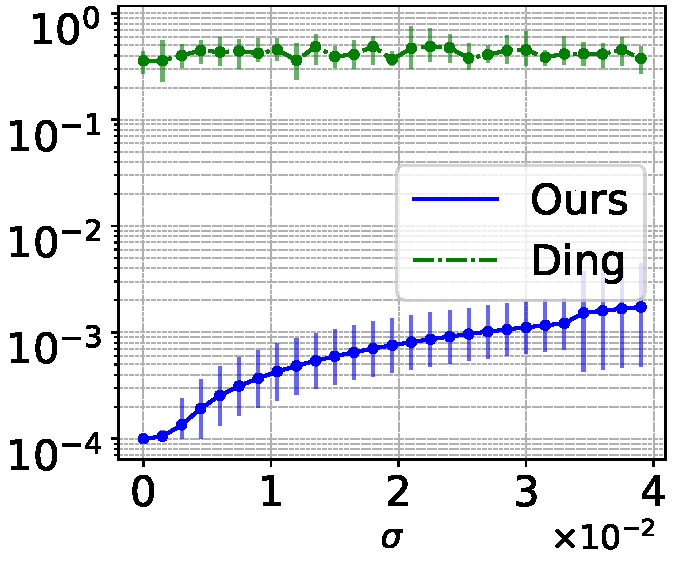
\includegraphics[width=0.28\linewidth]{images/compares/delta_f.pdf}
            \label{fig:delta_f}
            % \caption{Relative focal length error $\Delta f$ vs. noise level.}
        }
        \hfill
        \subfloat[$\Delta c$ vs. noise.]{
            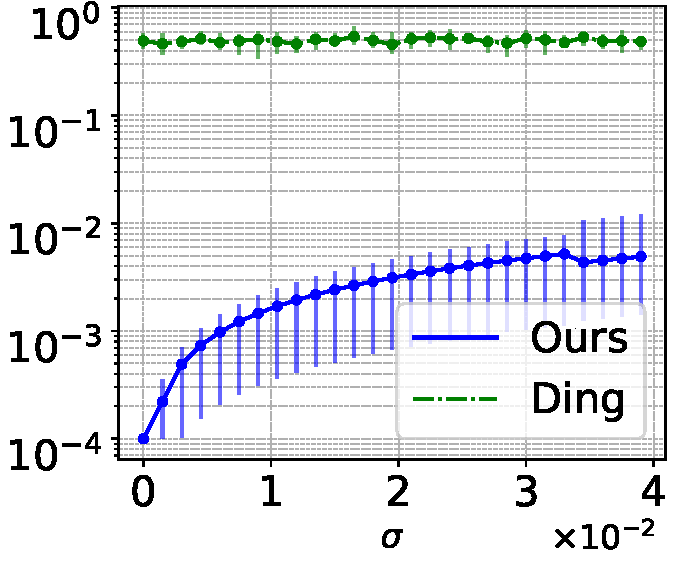
\includegraphics[width=0.28\linewidth]{images/compares/delta_uv.pdf}
            \label{fig:delta_uv}
            % \caption{Center offset error $\Delta c$ vs. noise level.}
        }
        \hfill
        \subfloat[$\Delta s$ vs. noise.]{
            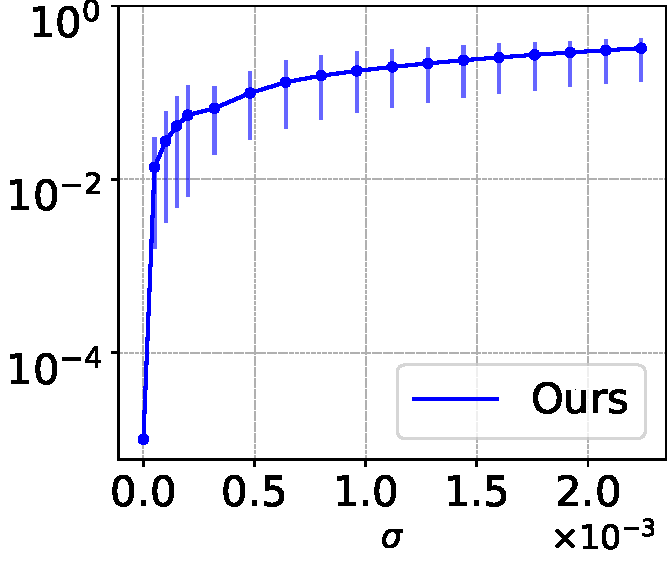
\includegraphics[width=0.28\linewidth]{images/compares/delta_skew.pdf}
            \label{fig:delta_skew}
            % \caption{Skew error $\Delta \alpha$ vs. noise level. A significant relative value error is present but the method shows resiliance w.r.t noise. }
        }
    

        \subfloat[$\Delta \RR$ (degrees) vs. noise.]{
            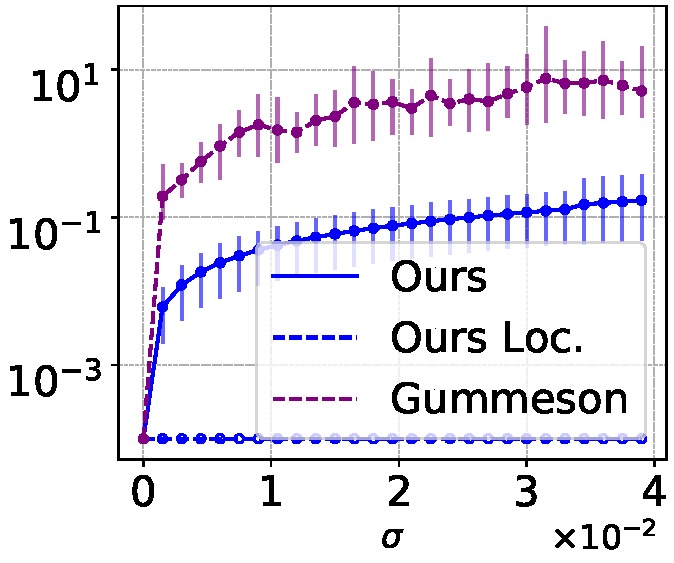
\includegraphics[width=0.28\linewidth]{images/compares/delta_r.pdf}
            \label{fig:delta_r}
            % \caption{Rotational error $\Delta R$ (degrees) vs. noise level.}
        }
        \hfill
        \subfloat[$\Delta \mathbf{t}$ vs. noise level.]{
            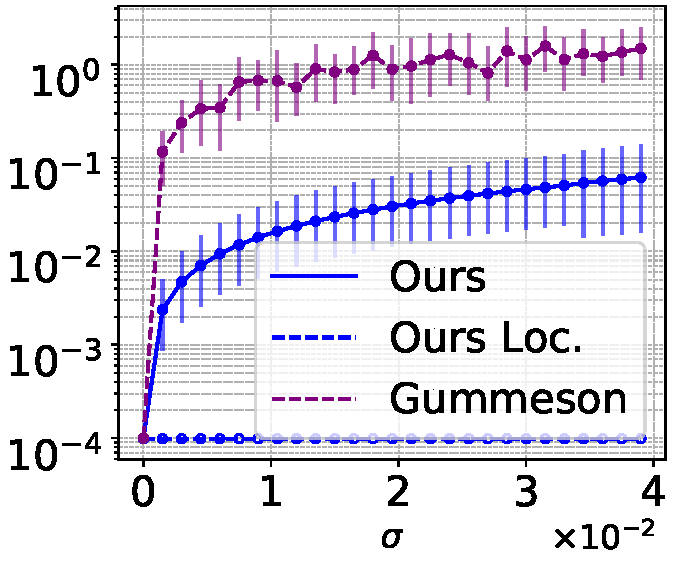
\includegraphics[width=0.28\linewidth]{images/compares/delta_t.pdf}
            \label{fig:delta_t}
            % \caption{Translation error $\Delta t$ vs. noise level.}
        }
        \hfill
        \subfloat[$\%$ of successful trials.]{
            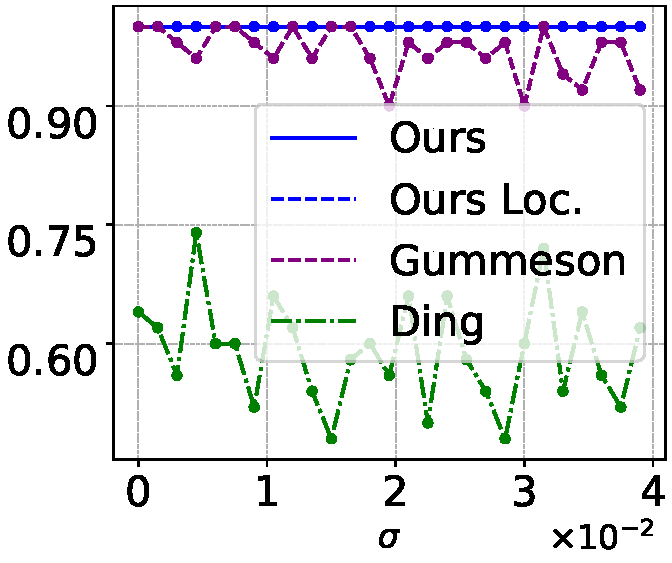
\includegraphics[width=0.28\linewidth]{images/compares/success_rate.pdf}
            \label{fig:success_rate}
            % \caption{Percentage of trials in which the method successfully found a solution.}
        }
    \caption{Results of our method on the two tasks of camera calibration (top row) and pose estimation (bottom row). In (f) we also report the success rate.}
    \end{figure}
    

\subsection{Results on rendered scene}

We further evaluated the proposed methods on a digital replica of a real scene, composed of three pipes around a corner. This setting is interesting since edge detection and pairing is as close as possible to a real scenario while still knowing ground truth. The scene is shown in Figure~\ref{fig:pipes}.

The pipes are assumed to be unitary radius, and meet at the world origin.

We assume the skew set to zero and use two view of the scene.
The estimated intrinsic parameters ($f_x = 2563.36$, $f_y = 2924.82$, $c_x = 518.657$, $c_y = 1242.12$) differ from ground truth ($f_x = 1500.00$, $f_y = 2666.67$, $c_x = 540$, $c_y = 960$) by a mean relative error of $28.5\%$.
The horizontal focal length $f_x$ contributes the most to this error, this is due to the fact that the algorithm has been initialized with a square aspect ratio as it is the most common case. Leveraging known at priori in this case would yield better results.

The reprojection error visualized in Figure~\ref{fig:pipes} shows that the estimated camera is very close to the ground truth.

For estimating the full camera parameters ($\KK, \RR,\mathbf{t}$), tracking all $59,\!049$ homotopy paths required 1 minute and 37 seconds.

\begin{figure}
    \centering
    \subfloat[Shot 1]{
        
\includegraphics[width=0.5\linewidth]{images/scenes/pipes/camera_1.png}
    }
    \subfloat[Shot 2]{
        
\includegraphics[width=0.5\linewidth]{images/scenes/pipes/camera_2.png}
    }
    \caption{Digital replica of a real scene, composed of three pipes around a corner. The scene is rendered in Blender and the camera is placed at the position of the real camera. Real borders as solid transparent lines, reconstructed borders as dashed lines.}
    \label{fig:pipes}
\end{figure}

\subsection{Results on real-world scenarios}

We further evaluated the proposed methods on 2 real-world scenarios. The first one is the same setting from Gummeson \cite{gummeson22pose} composed of supporting poles for a roller coaster. The second one is an office scene with three cylindrical markers arranged on a desk(Figure~\ref{fig:homotopy}).

\paragraph{Roller coaster}
The scene is composed of 6 poles, mostly verically aligned but not parallel. The original paper did not provide the actual radius but the cylinder matrices $\CC_i$ are available at \href{https://github.com/jo6815en/minimal_solvers_conics/blob/main/images/roller_coaster_data.mat}{Github}, as well as ground truth camera intrinsics and pose.

The estimated intrinsic parameters ($f_x = 1741.12$, $f_y = 1711.91$, $c_x = 918.0$, $c_y = 538.0$) differ from the ground truth ones ($f_x = 1749.83$, $f_y = 1751.29$, $c_x = 960.0$, $c_y = 540.0$) by a mean relative error of $2\%$.
The estimated camera pose ($R_x = -12.31$, $R_y = -1.50$, $R_z = -1.92$, $t_x = 2.90$, $t_y = -0.36$, $t_z = -0.36$) differs from ground truth one ($R_x = -11.89$, $R_y = -1.37$, $R_z = -2.15$, $t_x = 2.69$, $t_y =  0.07$, $t_z = -0.14$) by a mean relative error of $3.5\%$.

The reprojection error visualized in Figure~\ref{fig:roller_coaster} shows that the estimated camera is very close to the ground truth. The reprojection error is comparable to the one reported in Gummeson et al. \cite{gummeson22pose} and we achived that while also estimating intrinsic parameters.

\begin{figure}[h]
    \centering
    \subfloat[Gummeson et al. \cite{gummeson22pose}]{
        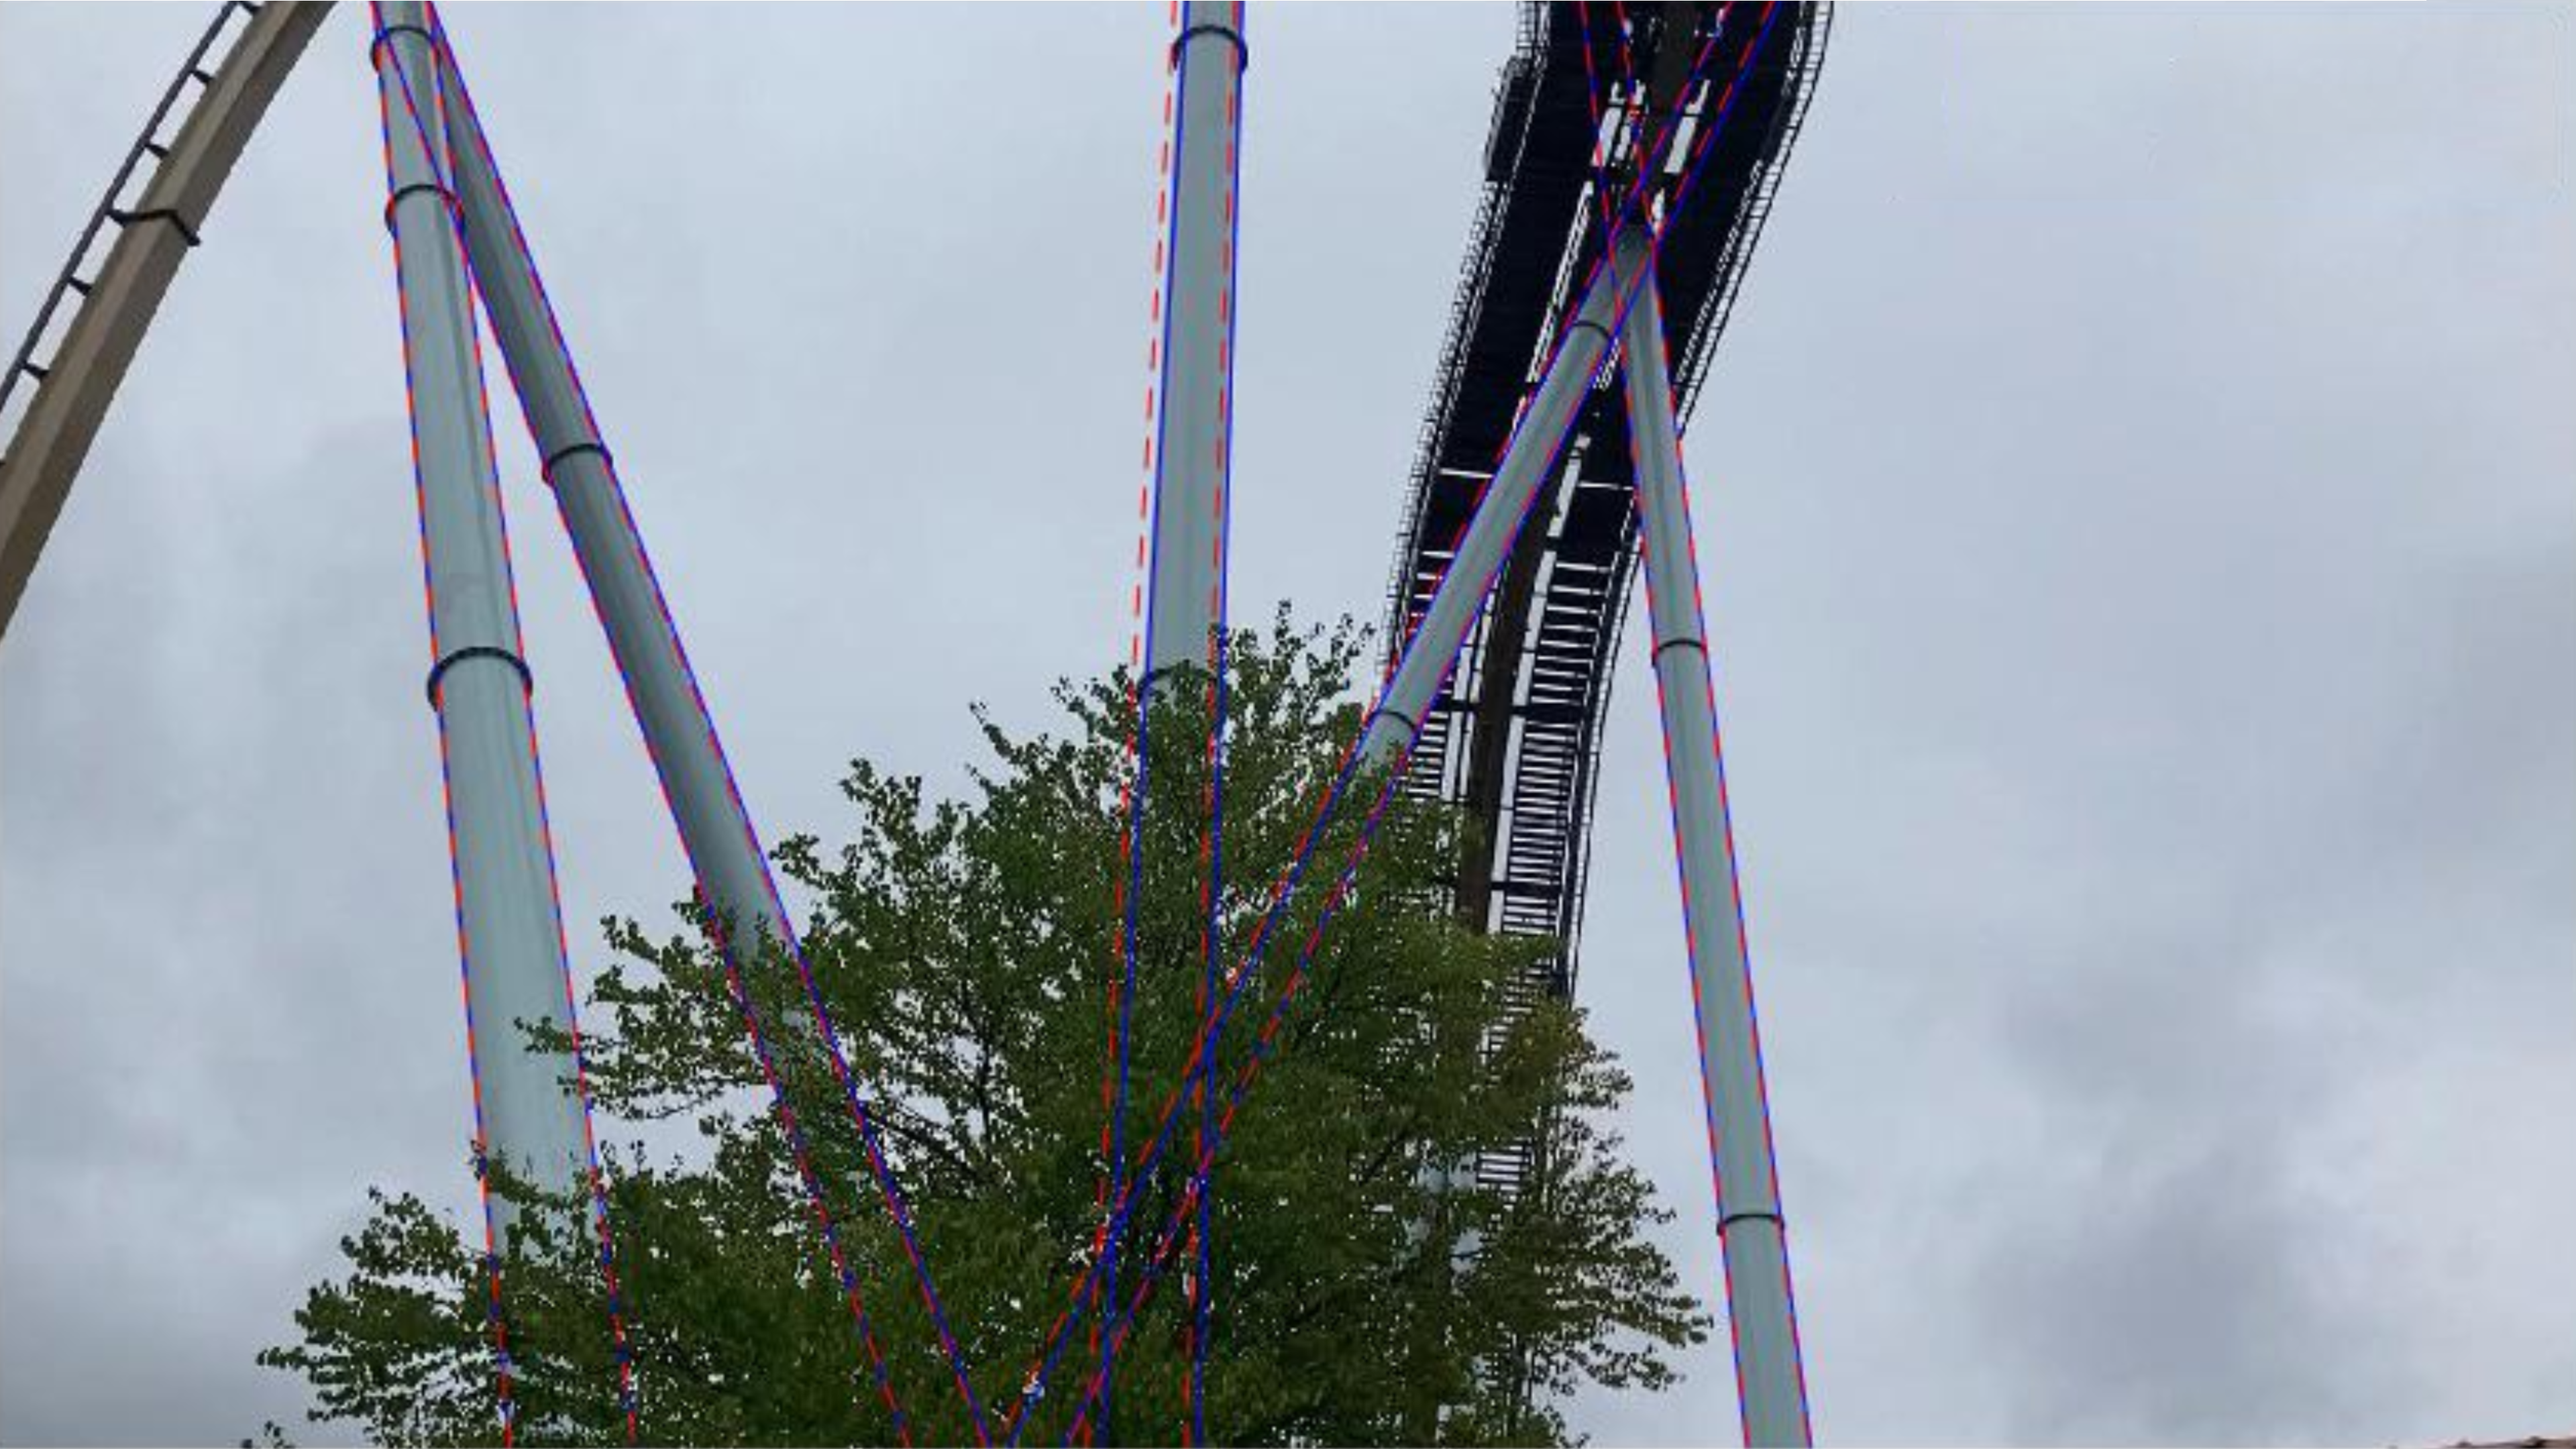
\includegraphics[width=0.5\linewidth]{images/scenes/roller_coaster/rollercoaster_gummeson.png}
    }
    \subfloat[Ours]{
        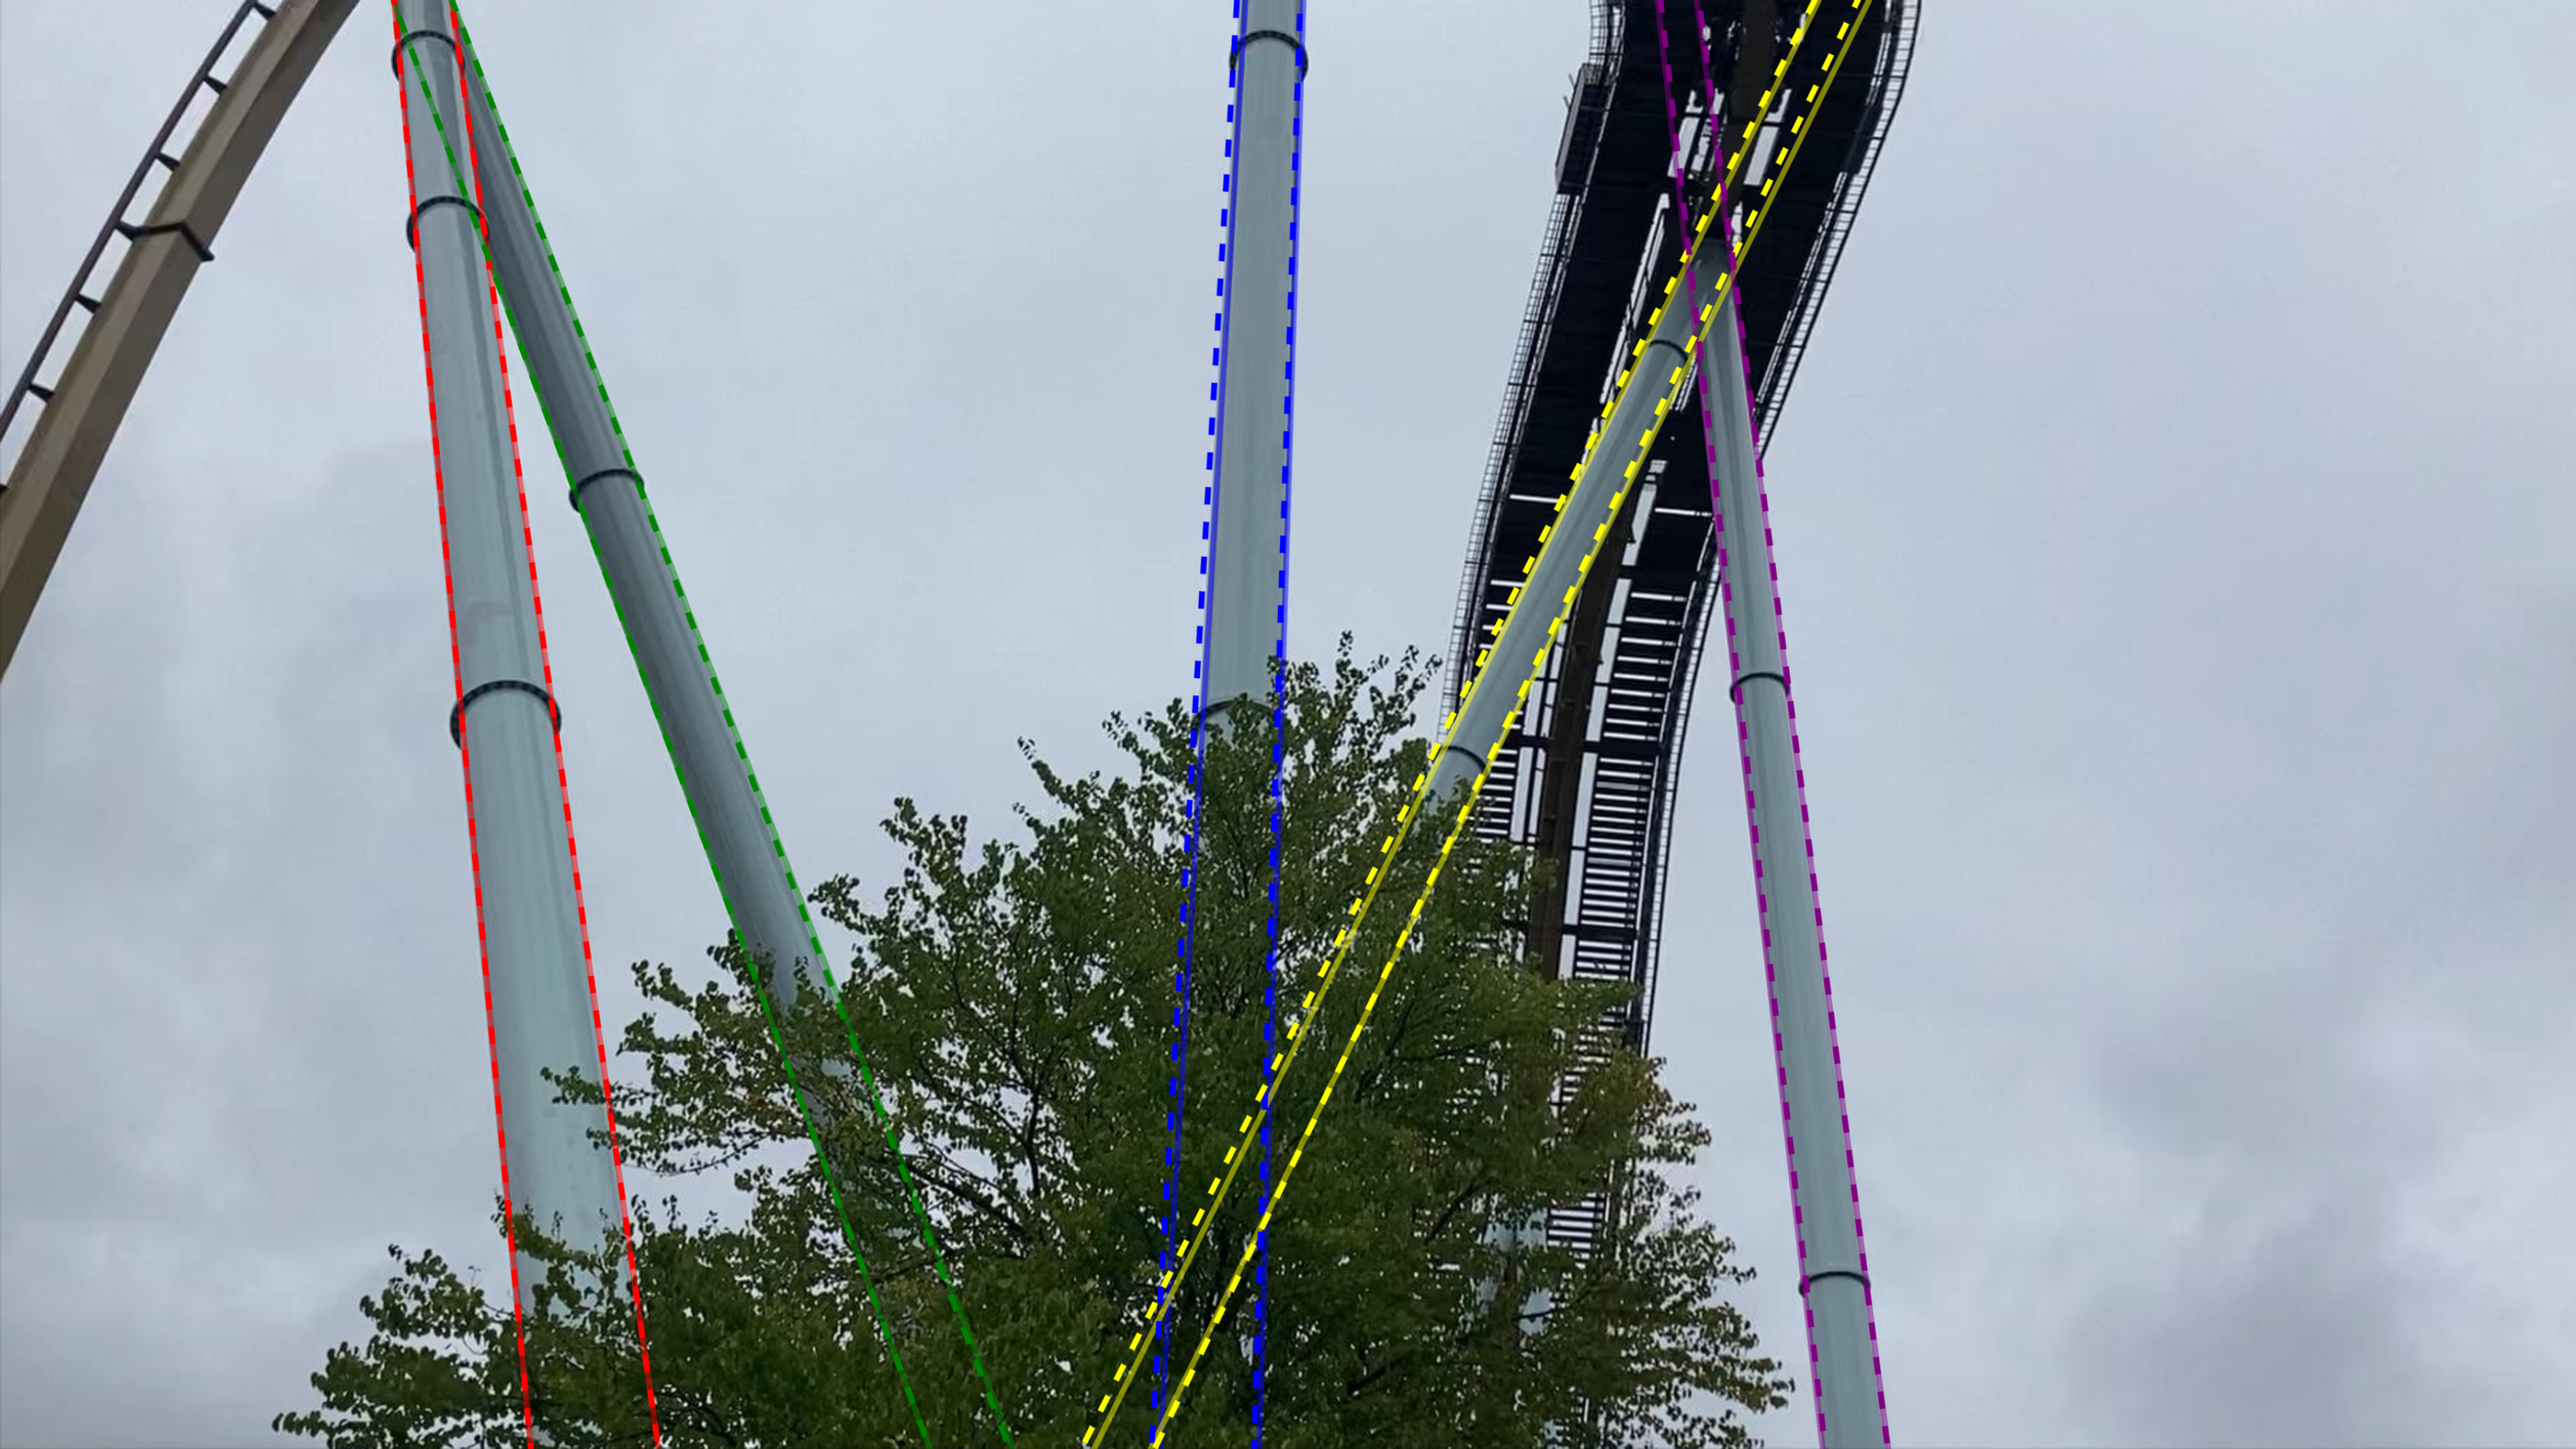
\includegraphics[width=0.5\linewidth]{images/scenes/roller_coaster/rollercoaster_ours.png}
    }
    \caption{Roller coaster scene from Gummeson et al. \cite{gummeson22pose}. We achieved a comparable reprojection error while estimating intrinsic parameters. Real borders as solid transparent lines, reconstructed borders as dashed lines.}
    \label{fig:roller_coaster}
\end{figure}

\paragraph{Markers}
Ground truth camera poses were estimated using \textsc{COLMAP}~\cite{schoenberger2016sfm, schoenberger2016mvs}.
The 3D position of the cylinders are known.

We assume the skew set to zero and use two view of the scene. The estimated intrinsic parameters ($f_x = 1334.72$, $f_y = 1234.91$, $c_x = 848.93$, $c_y = 960$) differ from the \textsc{COLMAP} results ($f_x = 1632.60$, $f_y = 1605.51$, $c_x = 540$, $c_y = 960$) by a mean relative error of $22\%$, which is still lower than the one achieved by  Ding et al.~\cite{CalibrationFreePlacedRightCylinder} on synthetic data
For localization, $\Delta \RR$ is computed on the relative pose of the two cameras and differs from ground truth by $2\%$. $\Delta \mathbf{t}$  differs by $9\%$.

For estimating the full camera parameters ($\KK, \RR,\mathbf{t}$), tracking all $59,\!049$ homotopy paths required 1 minute and 39 seconds.
Interestingly, once $\KK$ is estimated,  localization for additional frames requires tracking fewer parameters, resulting in improved speed and accuracy. Execution time drops below one second (single-threaded), with a relative rotation error of $2\%$ and translation error of $0.9\%$.% Furthermore, since subsequent frames can be processed independently, the method becomes suitable for real-time scenarios.

%-------------------------------------------------------------------------
